\begin{frame}
    \frametitle{AHTR Temperature Model}
    \begin{itemize}
        \item I used the open-source MSR simulation tool, Moltres, to conduct AHTR
        full assembly multiphysics simulations 
        \item AHTR Moltres simulations captures thermal feedback effects, absent
        from the purely neutronics OpenMC simulations
    \end{itemize}

    \begin{block}{Steps to produce Moltres AHTR Temperature Model}
        \begin{itemize}
          \item OpenMC neutronics model produces group constants data for the Moltres model
          \item Moltres model mesh generation
          \item Moltres temperature model accepts group constants data and mesh
        \end{itemize}
        \end{block}

    \begin{block}{Energy Homogenization}
        \begin{table}[]
            \centering
            \begin{minipage}[c]{0.6\textwidth}
                \centering
                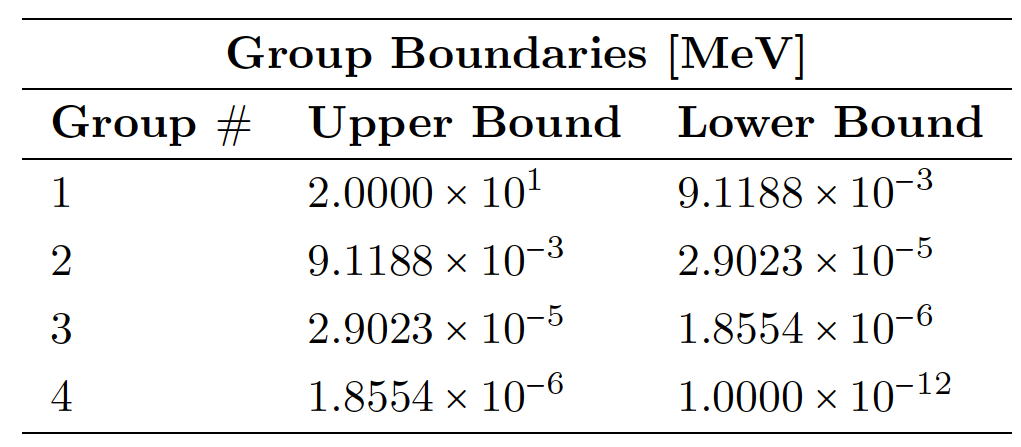
\includegraphics[width=0.7\linewidth]{figures/ahtr-energy-discr.png}
            \end{minipage}\hfill
            \begin{minipage}[c]{0.4\textwidth}
            \caption{4-group energy structures for AHTR geometry 
            derived by \cite{gentry_development_2016}.}
        \end{minipage}
        \end{table}
    \end{block}
\end{frame}

\begin{frame}
    \begin{block}{Spatial Homogenization}
        Fuel slab discretization into 13 cells: FLiBe, left graphite, right graphite, 
        and ten fuel cells (each cell has a different packing fraction)
    \end{block}
    \begin{figure}[]
        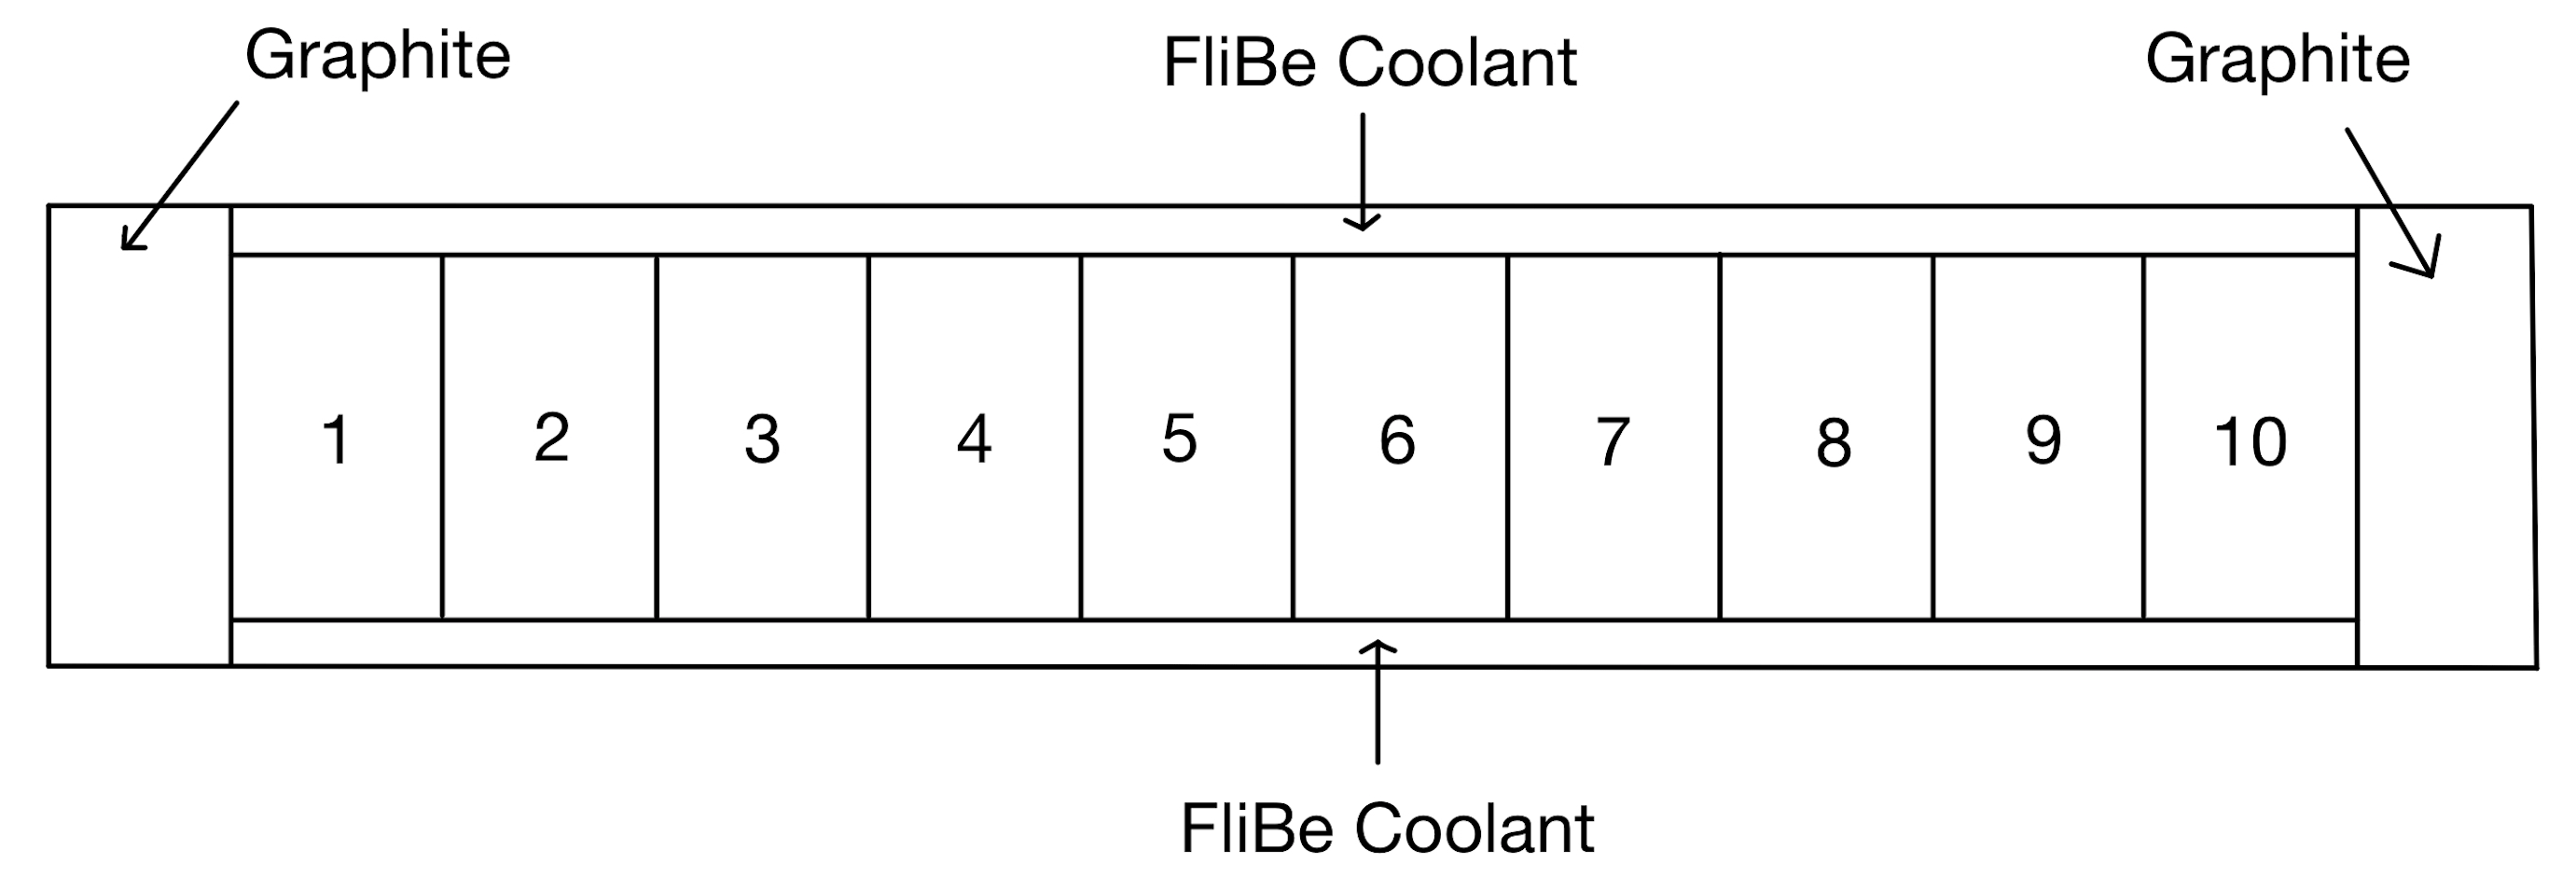
\includegraphics[width=0.8\linewidth]{figures/straightened_slab_mg.png}
        \caption{Straightened AHTR fuel slab spatially discretized into 
        13 \textit{cells} for OpenMC multigroup calculation.}
    \end{figure}

\end{frame}